%Chapter 3: Background
%1) Introduction paragraph summarizing the flow/content/structure of the Background chapter
%2) Radiometer Basics
%	a) Power Detection
%	b) Integration and filtering
%	c) Metrics
%		i) Sensitivity
%		ii) Stability
%	d) Implementation
%3) Software Defined Radio Basics
%	a) High-level figure of the components of a generic SDR.
%	b) SDR Operation
%	c) GNURadio Operation
%4) Software Defined Radio Development Platform (i.e. your specific platform)
%	a) Hardware (i.e. N200)
%	b) Software (i.e. GNU Radio)  

\chapter{BACKGROUND}\label{ch:background}
This chapter gives background information on the operation of  traditional radiometers and on software defined radios.  We begin by looking at the major components of a radiometer and how it measures power.  Next the metrics used to measure the performance of a traditional radiometer are discussed.  Then an overview of how software defined radios operate is given.  Finally, we review the tools used to develop a software defined radio based radiometer.  

\section{Radiometer Basics}\label{rad_basics}
A radiometer is a device designed to measure thermal electromagnetic emission by a material media due to the electron agitation within the material [\cite{ulaby}.  This electromagnetic emission is the thermal noise of the object and can be correlated to the physical temperature of the object[\cite{Nyquist1928thermal}].  Because of this correlation, the amount of noise received is called the noise temperature and it is measured in Kelvin. 

There are six stages common to all radiometers.  They are:

\begin{enumerate}
\item Source (antenna or $T_{A}$)
\item Bandwidth ($\beta$),
\item Amplification (Gain or $G$),
\item Power detection ($X^{2}$),
\item Data smoothing,
\item Output (Voltage, rQ, Kelvin).
\end{enumerate}

Figure \ref{trad_radiometer} illustrates how a signal propagates through a radiometer.  First, the signal from the source enters the antenna, $T_A$.  Next the signal is filtered to a set bandwidth, $\beta$.  This filtered signal is then amplified by Low Noise Amplifiers (LNAs) by a gain of $G$.  The power information is then extracted from the signal using a square-law detector, $X^2$.  This device is a diode that operates in the square law region.  While the diode is operating in this region, the output voltage is proportional to the square of the input voltage and is therefore proportional to the input power [\cite{Leinweber}].  The voltage output from the square-law detector is then smoothed using an integrator with an integration time $\tau$.  Finally, the integrated voltage signal is then measured and recorded.

{\begin{figure}[h!tb] 
\centering
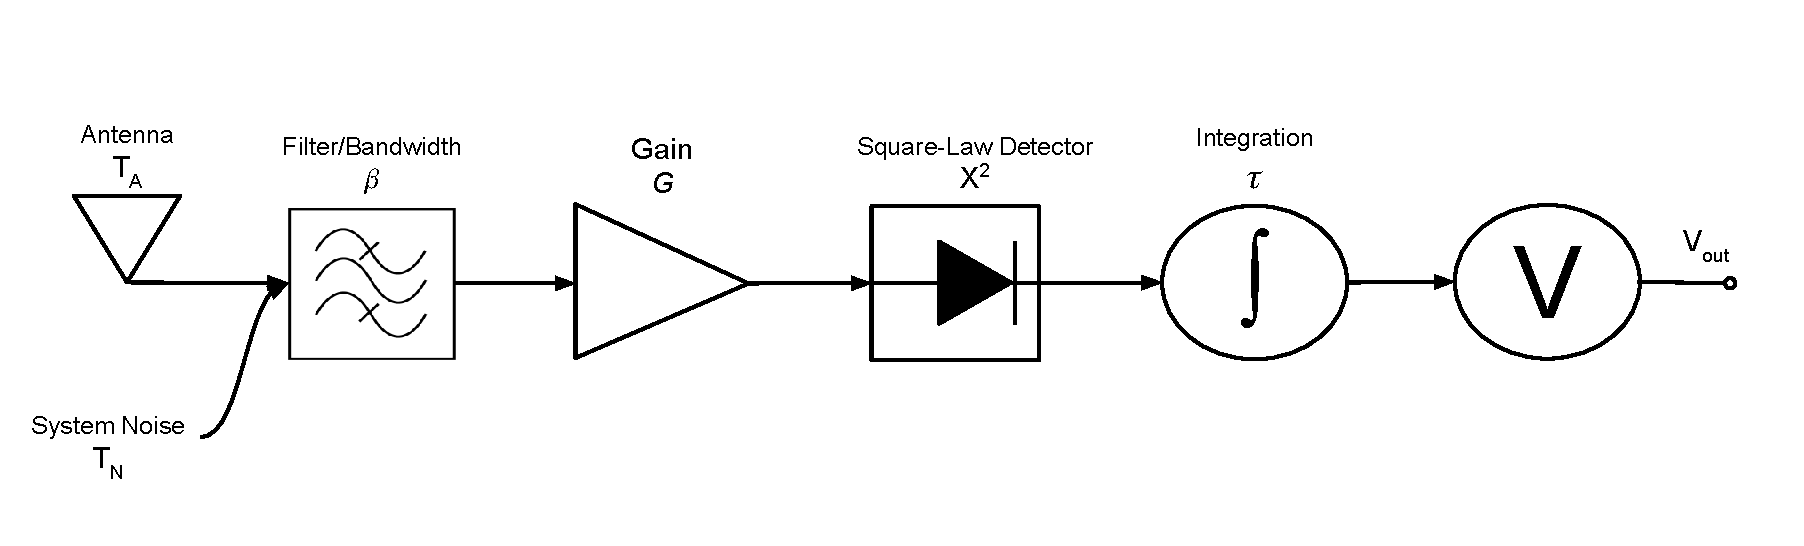
\includegraphics[width=\textwidth]{Images/Traditional_Radiometer.pdf}
\isucaption{A total power radiometer block diagram}
\label{trad_radiometer}
\end{figure}
}

A non-physical object that is present in all radiometers is system noise, represented as $T_{N}$.  System noise is noise that is generated from within the radiometer due to thermal agitation.  A radiometer is designed to reduce system noise as much as possible by using low-loss components and amplifiers that are low noise, such as Low Noise Amplifiers (LNAs). 

\subsection{Power Measurement}\label{pwr_measurement}

As shown in Equation \ref{eq:power_rad_eq}, the power measured by an ideal radiometer is equal to the product of the power received from the source ($T_A$), the gain ($G$) and the bandwidth ($\beta$) of the radiometer, and the Boltzmann constant ($k=1.38 x 10^{-23} J/K$).

\begin{equation} \label{eq:power_rad_eq}
P=k*\beta*G*(T_{A})\ watts
\end{equation}

While the components of an ideal radiometer do not contribute noise power ($T_N$) to the system, they do in a real radiometer.  The impact of this internally generated and unwanted noise on the power measured by the radiometer is captured by Equation \ref{eq:final_power}.

\begin{equation} \label{eq:final_power}
P=k*\beta*G*(T_{A}+T_{N})\ watts
\end{equation}

Gain ($G$) and bandwidth ($\beta$) are important design parameters of a radiometer.  While a large gain is desired to amplify the source signal ($T_A$), the magnitude of the gain must be limited since it also amplifies the unwanted system noise ($T_N$).

The bandwidth of the source signal is typically wide (large) to maximize the power measured by the radiometer.  The two primary limiting factors to bandwidth are: 1) hardware limitations (e.g. LNA operating limits), and 2) unwanted signals located at a number of frequencies (e.g. radio communication signals).

\emph{Low Noise Amplification.}  The method used by most radiometers to mitigate the system noise contributed during signal amplification is daisy chaining (i.e. cascading) devices called Low Noise Amplifiers (LNAs).  The total amount of amplification we can expect from $n$ LNAs that are cascaded is the sum of the gain of each LNA shown in equation \ref{gain_sum}.

\begin{equation}\label{gain_sum}
G_{total}=G_1 + G_2 + G_3 + \cdots +G_{n-1}\ \ dB
\end{equation}

A performance metric of an LNA is the noise figure ($NF$).  The noise figure gives us the difference between the actual noise output and an ideal amplifier with the same gain and bandwidth attached to a matched load at the standard noise temperature (290 K).  Another metric used is the noise factor ($F$).  The noise factor is the ratio of the output noise power to the input noise power.  The noise factor (F) is related to the noise figure (NF) as shown in Equation \ref{noise_figure}.

\begin{equation}\label{noise_figure}
NF=10 * \log_{10}(F)\ \ dB
\end{equation}

For devices that are cascaded, the total noise factor is found by the Friis formula and results in equation \ref{noise_factor}.  

\begin{equation}\label{noise_factor}
F=F_1+\frac{F_2-1}{G_1}+\frac{F_3-1}{G_1 G_2}+\frac{F_4-1}{G_1 G_2 G_3}+\cdots +\frac{F_n-1}{G_1 G_2 G_3 \cdots G_{n-1}}
\end{equation}

The key implication is that the first LNA in the cascade contributes the most system noise.  As a consequence, it is critical that the first LNA has the smallest noise factor, while the remaining LNAs provide a majority of the signal gain.

\subsection{Radiometer Performance Metrics}\label{performance_metrics}

Two criteria used to determine how well a radiometer performs are: 1) Sensitivity and 2) Stability.  These criteria determine the smallest change in signal noise temperature (i.e. power) the radiometer can detect, and the amount of drift power measurements have over an extended period of time, respectively..

\emph{Sensitivity}.  Sensitivity of a radiometer is the smallest change in power that can be detected.  A radiometer must be able to differentiate between signal noise received by  the antenna ($T_{A}$) and the system generated noise ($T_N$).

Two methods to quantify the sensitivity of a radiometer are: 1) experimentally, and 2) analytically.  Experimentally, sensitivity can be computed as the standard deviation of the measured power (assuming a stable radiometer).  Analytically, sensitivity can be computed as a function of radiometer properties defined in Equation \ref{NEAT_EQ}.  The term Noise Equivalent Delta ($\Delta$) Temperature ($NE\Delta T$) is often used interchangeably with sensitivity.  As can be seen in Equation \ref{NEAT_EQ}, sensitivity improves (i.e. becomes smaller) as the bandwidth ($\beta$) and/or integration time ($\tau$) of the radiometer increases[\cite{ulaby}].

\begin{equation} \label{NEAT_EQ}
NE\Delta T=\frac{T_{A}+T_{N}}{\sqrt{\beta * \tau}} 
\end{equation}

The following example illustrates the impact system generated noise has on a radiometers ability to detect changes in signal noise.  Lets assume we want a sensitivity of 1 K.  If there is no system generated noise (i.e. $T_N = 0$) and the received signal at the antenna is 200 K (i.e. $T_A = 200$), we can then calculate our receiver sensitivity by using Equation \ref{NEAT_EQ}.  Lets assume a bandwidth of 10 MHz (i.e. $\beta = 10 x 10^6$) and that our integration time is 40 milliseconds (i.e. $\tau = 0.04$).  We can now take these values and put them in Equation \ref{NEAT_EQ} which results in Equation \ref{NEAT_EX1}.

\begin{equation} \label{NEAT_EX1}
NE\Delta T=\frac{200 + 0}{\sqrt{10 x 10^6 * 0.04}} = 1 K 
\end{equation}

Equation \ref{NEAT_EX1} gives us a result of 1 K for our sensitivity, which meets our goal.  Because we do not have an ideal radiometer (i.e. $T_N \neq 0$), lets assume our system noise is 800 K (i.e. $T_N = 800$).  Assuming that our bandwidth ($\beta$), our integration time ($\tau$) and our antenna signal ($T_A$) is the same, we can now apply Equation \ref{NEAT_EQ}, which results in Equation \ref{NEAT_EX2}.  This results in a sensitivity of 5 K, which is five times higher than our ideal sensitivity of 1 K. 

\begin{equation} \label{NEAT_EX2}
NE\Delta T=\frac{200 + 800}{\sqrt{10 x 10^6 * 0.04}} = 5 K 
\end{equation}

As can be clearly seen, system noise makes the job of detecting changes in signal noise more difficult[\cite{skou}].  Section \ref{Exp2_analysis} uses both the experimentation and analytical methods of finding sensitivity as a cross validation of the correctness of our SDR based radiometer.

\emph{Stability.}  Stability of a radiometer is a measure of the degree to which fluctuations we see are a result of the source and not a change occurring within the radiometer.  Lets examine Equation \ref{eq:final_power}, which defines the total power the radiometer receives.  If our bandwidth ($\beta$), Gain ($G$), system noise ($T_N$), and Boltzmann constant ($k$) are constant, then the system is stable.  If we can assume that our bandwidth is fixed and that our system noise (mean value) is constant, then this leaves our Gain ($G$) being the uncertain variable that may cause unwanted fluctuations[\cite{Evans}]. 

Radiometer instabilities are due to Low Noise Amplifier (LNAs) gain fluctuations.  Two factors cause these gain fluctuations: 1) fluctuations in the LNA's voltage supply, and 2) fluctuation in the LNA's physical temperature.  

The impact these gain fluctuations have on stability is given by Equation \ref{eq:rad_stability}.  Where:

\begin{itemize}
\item $\Delta T_G$ is the noise temperature fluctuation,
\item $\Delta G$ is the LNA gain fluctuation,
\item $G$ is the ideal gain of the LNA and,
\item $T_{sys}$ is the combined antenna source ($T_A$) and system noise ($T_N$).
\end{itemize}

\begin{equation} \label{eq:rad_stability}
\Delta T_G=T_{sys} \left(\frac{\Delta G}{G}\right)
\end{equation}

These gain fluctuations can be controlled by closely monitoring and controlling both the voltage supply and temperature of the LNAs. However, this adds levels of complexity to the radiometer that may be impractical in some cases.  As an alternative, modifications to the basic radiometer given in Figure \ref{trad_radiometer} have been developed to compensate for these fluctuations.  There are three common types of radiometers designed to account for gain fluctuations.  They are: Dicke, Noise injection, and Polarimetric (or Correlating) radiometers.

\emph{Dicke Radiometer.}  Figure \ref{dicke_radiometer} shows the block diagram of a Dicke radiometer, which switches between measuring the source signal ($T_A$) and a known reference signal ($T_R$)[\cite{Dicke}].  By quickly switching between the source and reference signal at a frequency of $F_S$, a Dicke radiometer can reduce the impact of gain fluctuations on its stability.  

{\begin{figure}[h!tb] 
\centering
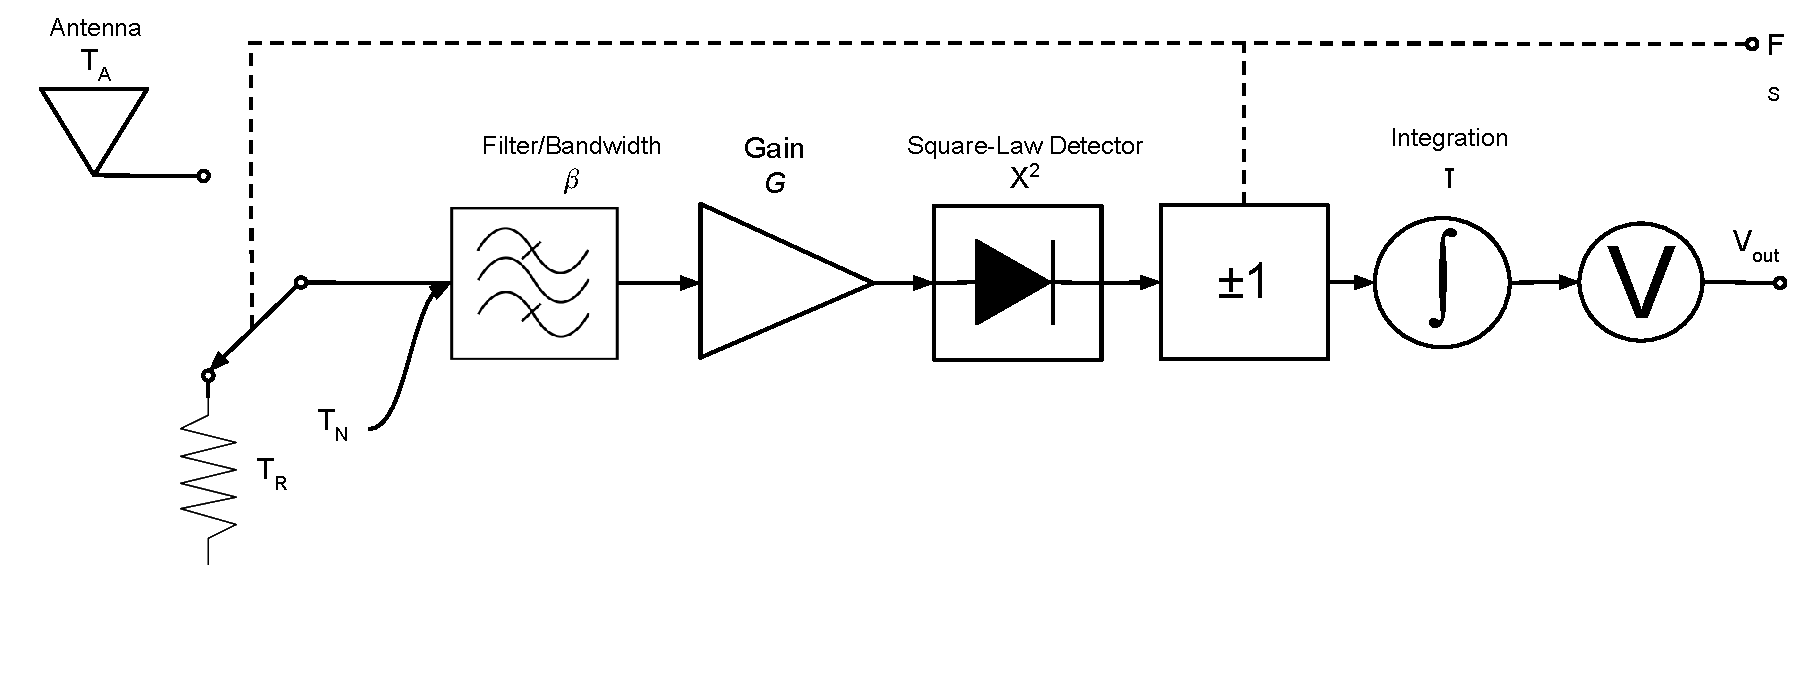
\includegraphics[width=\textwidth]{Images/Dicke_Radiometer.pdf}
\isucaption{A block diagram of a Dicke radiometer}
\label{dicke_radiometer}
\end{figure}
}

While a Dicke radiometer improves stability, it does so at the cost of not seeing the object of interest while it is measuring the reference signal.  This reduces the sensitivity of the radiometer, since the source signal is only observed for a fraction of the time.

{\begin{figure}[h!tb] 
\centering
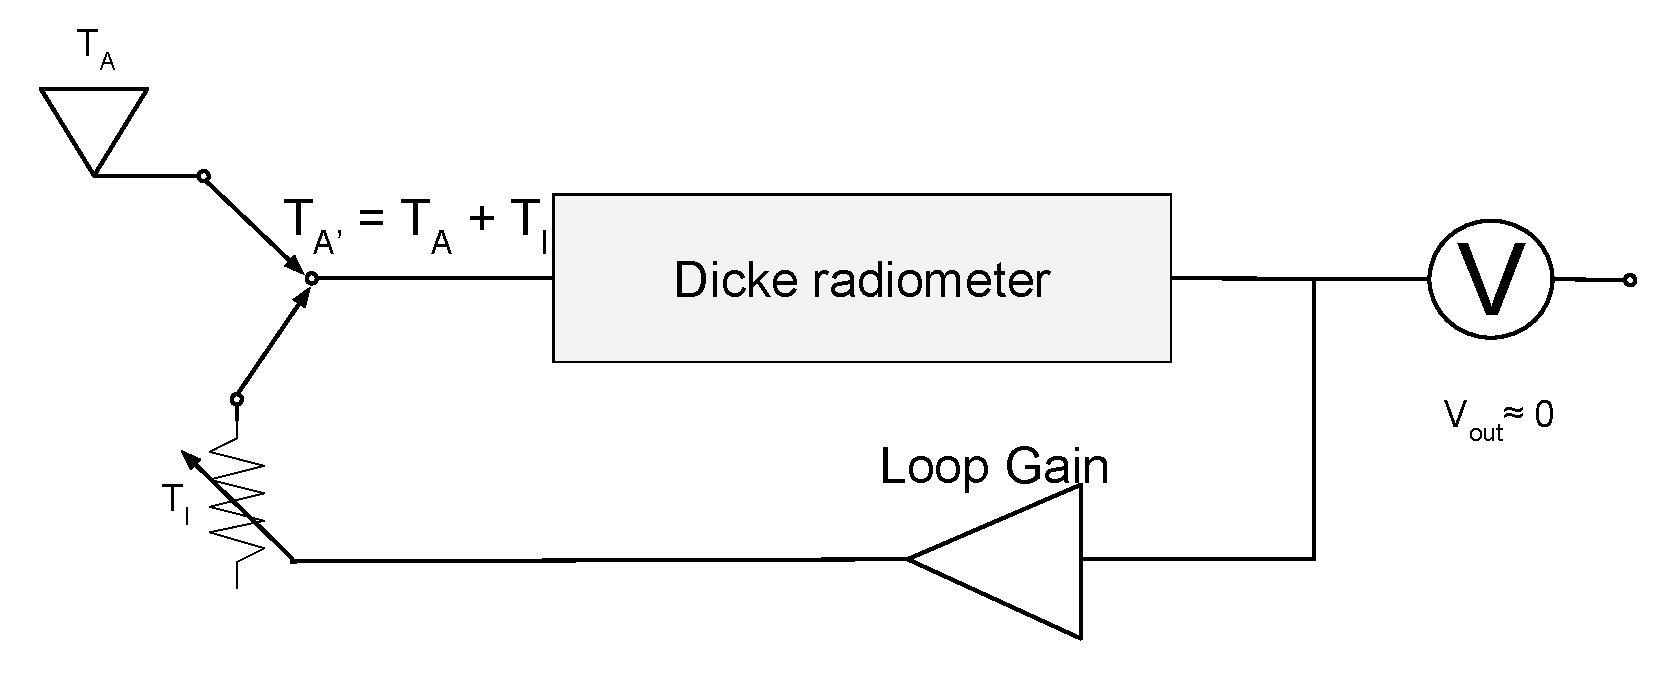
\includegraphics[width=\textwidth]{Images/Noise_inj_radiometer.pdf}
\isucaption{A block diagram of a Noise Injection radiometer}
\label{NoiseInj_radiometer}
\end{figure}
}

\emph{Noise Injection Radiometer.}  A noise injection radiometer is a variation of the Dicke radiometer, where a variable noise signal ($T_I$) is injected into the RF chain, as shown in Figure \ref{NoiseInj_radiometer}.  The injected noise signal power is adjusted so when added to the source signal their sum equals the reference signal power.  This improves stability by eliminating gain fluctuations, but increases system noise ($T_N$), which reduces radiometer sensitivity.

\emph{Polarimetric Radiometer.} A polarimetric (or correlating) radiometer uses two polarized signals, referred to as vertically polarized (V-Pol) and horizontally polarized (H-Pol).  In order to accomplish this, an antenna with dual polarization is used [\cite{Fujimoto}].  Each polarized signal is fed into the radiometer and correlated.  Because the source noise signal has polarization and the gain fluctuations do not, the gain fluctuations can be eliminated.  This reduces gain fluctuations to increase stability, while helping maintain sensitivity.  However, this is at the cost of increasing radiometer complexity and price, since two identical receivers (one for each polarization) are required. 
 
\section{Software Defined Radios Basics} 
A Software Defined Radio (SDR) is a device that digitizes a received RF signal as soon as possible, and processes the digital representation of the signal using a computer, FPGA, or dedicated System on Chip (SoC).  A canonical software defined radio architecture consists of a power supply, antenna, analog to digital converter, and a processing unit to carry out radio functions in software [\cite{Mitola1995}]. An ideal software defined radio block diagram is shown in Figure \ref{ideal_sdr}.

{\begin{figure}[h!tb] 
\centering
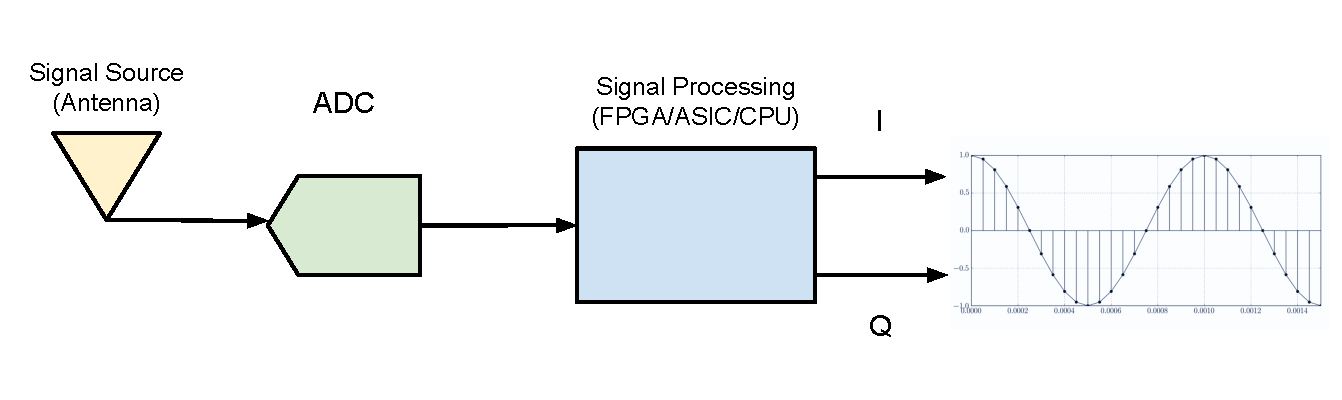
\includegraphics[width=\textwidth]{Images/SDR_Ideal_block.pdf}
\isucaption{An ideal software defined radio}
\label{ideal_sdr}
\end{figure}
}

A SDR can perform certain hardware functions in software (e.g. filtering), which provides flexibility over hardware solutions.  Changes can be made by simply uploading new software or firmware to the system.  This has a cost benefit as certain hardware components are no longer needed, and changes made in software do not require hardware to be added, removed or modified.

A more realistic software defined radio is shown in Figure \ref{prac_sdr}, where two items have been added.  First, an amplification of the signal (gain) is added to ensure the signal can be detected.  Second, a mixer is often used to down-convert the high frequency RF source signal to a lower frequency so a less expensive analog to digital converter can be used.  However, if the source signal frequency is already within the range of the analog to digital converter, then the mixer may be omitted.   

{\begin{figure}[h!tb] 
\centering
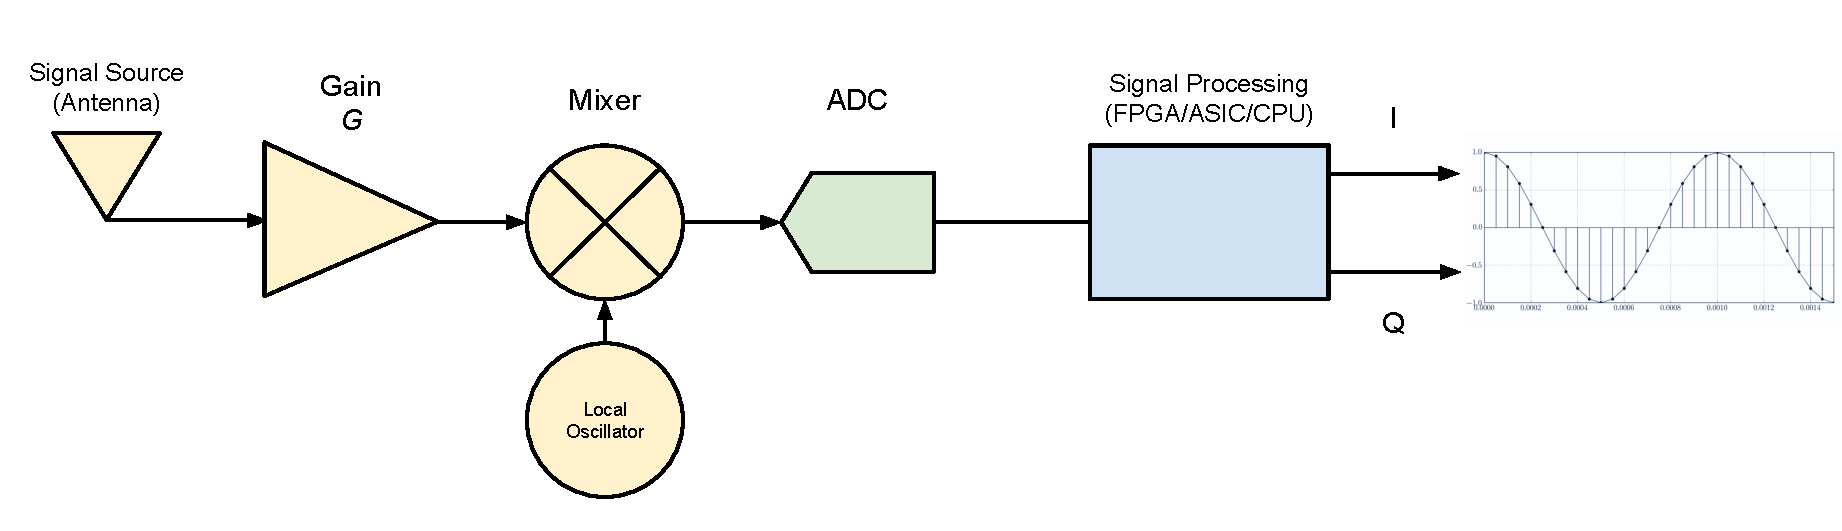
\includegraphics[width=\textwidth]{Images/SDR_Prac_block.pdf}
\isucaption{A typical software defined radio}
\label{prac_sdr}
\end{figure}
}

\emph{Software Defined Radio Applications.}  Software Defined Radios (SDRs) can be used for a variety of applications, but have been primarily used in the area of communications.  Some examples of these applications include:  mobile communications, wireless local area networks, personal area networks, and digital broadcast.  They appeal to applications where having the ability to change a modulation scheme or filter on the fly is desirable.  In these respects, SDRs often outperform traditional hardware-only radios because of their ability to easily change their operations through software.  

Early SDRs were expensive due to the cost of high speed analog to digital converters (ADCs) and high-end Field Programmable Gate Arrays (FPGA) that were required.  In recent years, the cost of SDRs have decreased due to the cost of these key components decreasing.  Also, while the cost of SDRs has gone down, their performance has increased.  This has led to SDRs becoming feasible for use in many new ways [\cite{jondral2005software}].

\section{Software Defined Radio Development Platform} \label{SDR_platform}
This section discusses the platform used to develop a software defined radio based radiometer.  The hardware and software tools used are off the shelf.  First, the hardware platform will be introduced, followed by the software platform.  

\subsection{Hardware Platform}\label{N200_HW}
The hardware platform selected for this work is the Ettus Research Group N200 SDR shown in Figure \ref{N200}.  The N200 has the following features that made it desirable for our specific application:

\begin{itemize}
\item Dual 14-bit ADC,
\item 25 MHz bandwidth per channel,
\item Modular daughter-board system for RF front end.
\end{itemize}

Its flexible architecture and ability to support a large bandwidth made the N200 an ideal hardware platform for software defined radio based radiometer development.

{\begin{figure}[h!tb] 
\centering
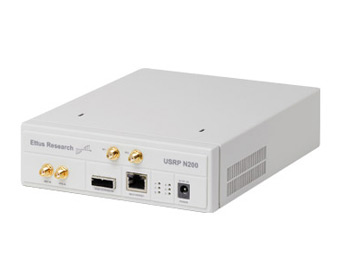
\includegraphics[width=7cm]{Images/n200}
\isucaption{The USRP N200 from Ettus Research (Image from Ettus Research Website - www.ettus.com)}
\label{N200}
\end{figure}
}

When selecting the hardware for this thesis, the requirements defined in Section \ref{requirements} were examined.  The bandwidth requirement was a deciding factor for hardware selection.  It was decided that a minimum bandwidth of 20 MHz was desired.  The 14-bit ADC was not a defined requirement, but was deemed to provide an adequate level of resolution.  The N200 has a flexible architecture through the use of daughter-boards.  

Figure \ref{N200_block} shows the overall architecture of the N200 SDR.  A daughter board directly receives the RF signal and then outputs analog I (in-phase) and Q (quadrature phase) signals that are then sampled by the N200 14-bit  A/D converter.

{\begin{figure}[h!tb] 
\centering
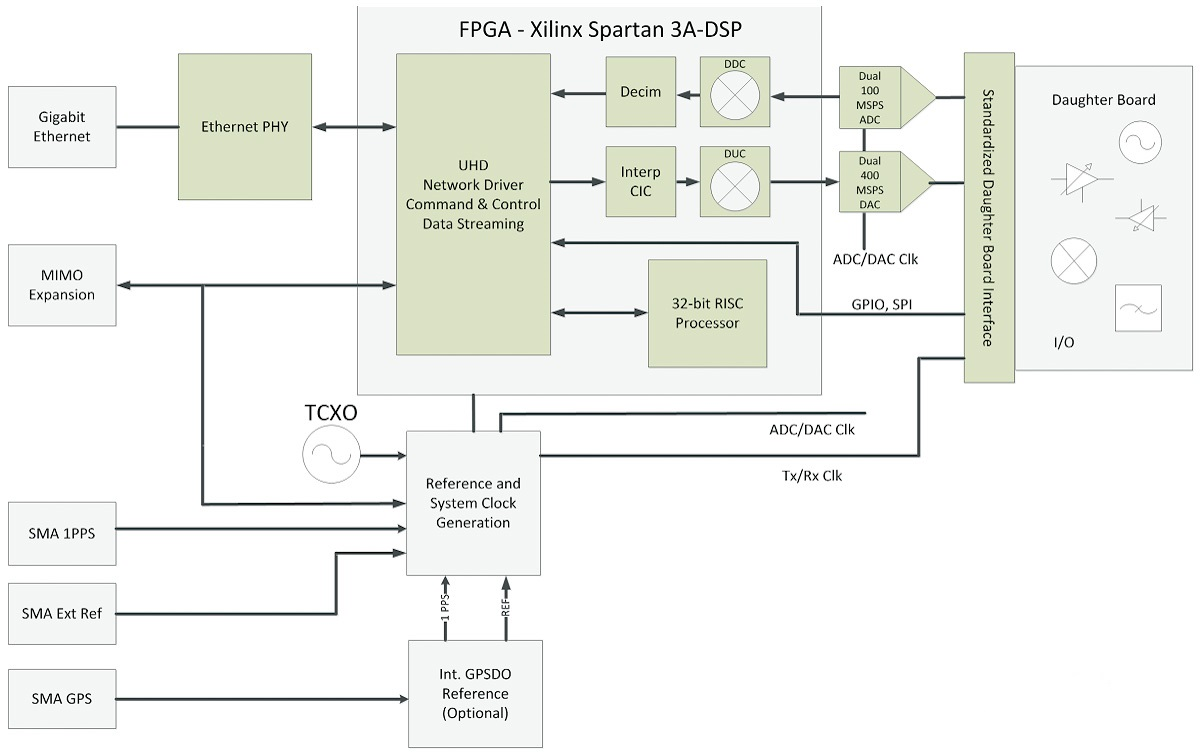
\includegraphics[width=14cm]{Images/n200_block_edited}
\isucaption{A block diagram of the Ettus N200 SDR. (Image from Ettus Research Website - www.ettus.com)}
\label{N200_block}
\end{figure}
}

\emph{The DBSRX2 Receiver.}  The daughter board selected for this work was the DBSRX2, shown in Figure \ref{dbsrx2}.  This daughter board is receive only, and operates between 800 MHz and 2400 MHz, which includes the frequency band required for this work (1400 MHz - 1425 MHz).

{\begin{figure}[h!tb] 
\centering
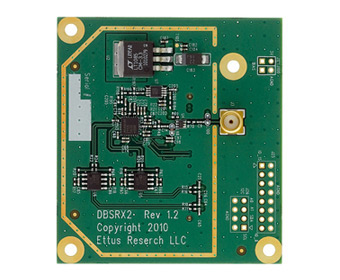
\includegraphics[width=7cm]{Images/dbsrx2.jpg}
\isucaption{The DBSRX2 daughter board from Ettus Research (Image from Ettus Research Website - www.ettus.com)}
\label{dbsrx2}
\end{figure}
}

The DBSRX2 has the RF hardware needed to transform the received RF signal into in-phase and quadrature-phase outputs.  This includes a programmable gain amplifier, a direct-conversion converter, a mixer, and finally a band-pass filter.  Figure \ref{dbsrx2_block} provides a block diagram of the DBSRX2.  First, the signal received is amplified by the Programmable Gain Amplifier (PGA).  The PGA can be configured by software.  Next, the signal goes into a direct-conversion integrated circuit (a Maxim 2112).  This integrated circuit directly converts the RF signal into analog I (in-phase) and Q (quadrature phase) signals and is composed of an integrated mixer and band-pass filter.

{\begin{figure}[h!tb] 
\centering
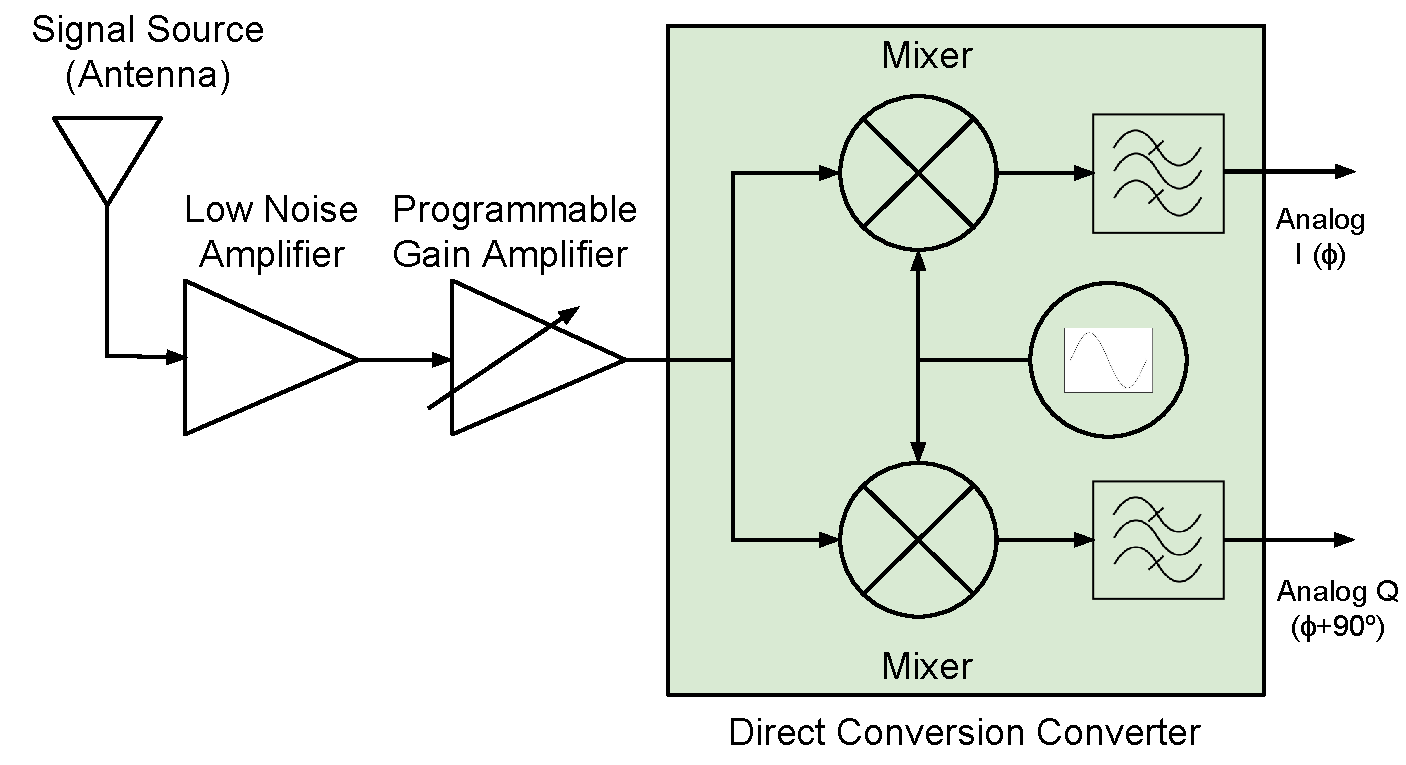
\includegraphics[width=12cm]{Images/DBSRX2_block.pdf}
\isucaption{Block diagram of the DBSRX2 daughter board.}
\label{dbsrx2_block}
\end{figure}
}

These analog I and Q signals are then sent to the analog to digital converter to be digitized.  The IQ signal are transmitted as differential signals to minimize noise.  Once digitized, the digital I-Q values are sent to a FPGA to be processed, and then sent to the PC for software based signal processing.

\subsection{Software Platform} \label{software_platform}

There are two pieces of software that are used with the software defined radio:  1) the firmware that is used in the FPGA of the N200, and 2) the software running on the host PC.  

The firmware provides low level processing of the signal before being sent to the software located on the PC.  It also provides a link for controlling key aspects of the software defined radio, such as gain, bandwidth and the center frequency.  This firmware comes pre-loaded into the FPGA by Ettus Research, and can be upgraded using tools provided by Ettus Research.

The software on the host PC performs signal processing on the I/Q data.  GNURadio was selected to be this software.   GNUradio is an open source software package designed for software defined radio application development.  It provides a GUI framework to create an interactive environment for the user, and is well supported by the N200 hardware.  

GNURadio uses a combination of Python and C++, where Python handles the high level interface and C++ is used to implement drivers and low level interfaces to the hardware.  This combination allows for a system that is easy to use, but still meets the performance required for handling large amounts of data. 

GNURadio also has a rapid development tool called GNURadio companion (GRC).  GRC is a simple to use graphical system for designing and building radio components in software. An example of GRC is shown in Figure \ref{N200_GRC}.

{\begin{figure}[h!tb] \centering
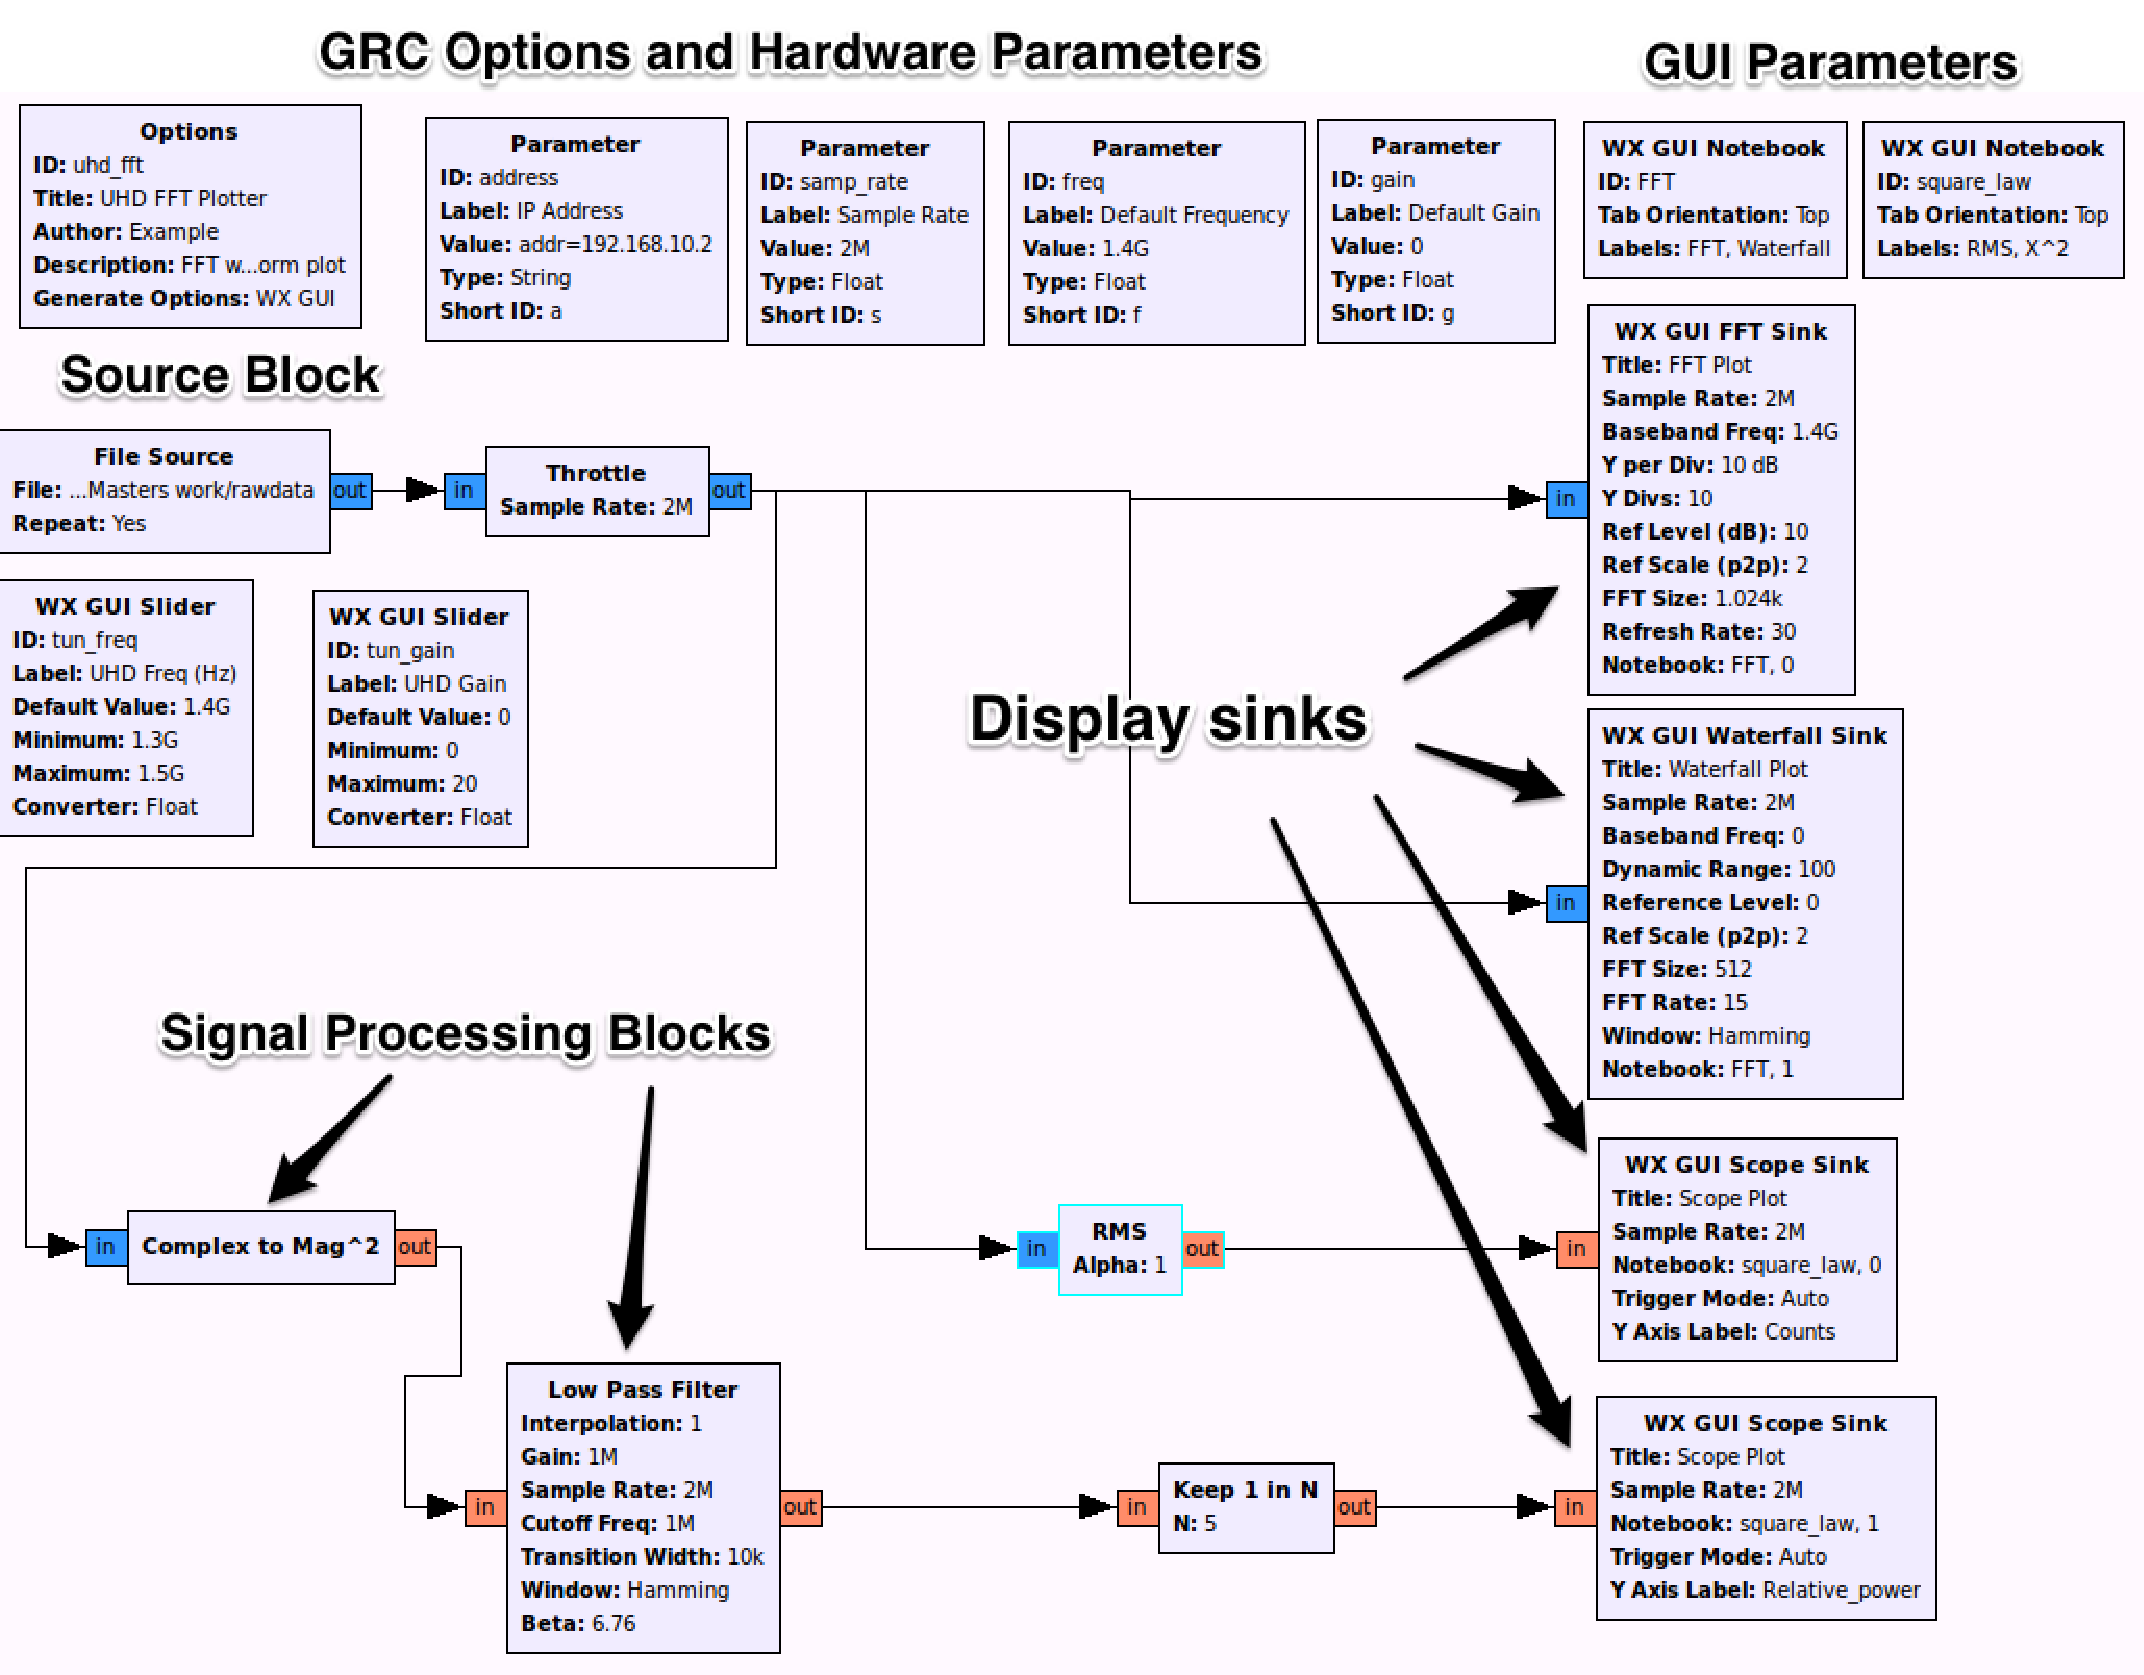
\includegraphics[width=\textwidth]{Images/radiometer_power_grc.pdf}
\isucaption{A screenshot of the GNURadio Companion editor program.  Source:  GNURadio}
\label{N200_GRC}
\end{figure}
}

GNURadio Companion provides common functions, such as signal sources, signal processing and signal sinks, as blocks that can be picked and placed on the screen.  Once placed, the blocks can be wired up, much like in LabView, and the flow of data can be controlled in this fashion.  GNURadio Companion also includes blocks that allow for building a GUI interface, which can be used to display data and control the software defined radio.

If a block does not exist, it can be created.  Because GNURadio uses Python, users can use this powerful and flexible language to build new blocks that can be imported into GRC.    

Using GNURadio and GNURadio Companion, a software defined radio can be rapidly built with little programming experience.  The excellent support of the hardware selected, and the ease of use made it an ideal development tool for building the necessary software for our SDR-based radiometer.

%----------------------------------------------------------
% End of Chapter 3.  Anything below this is extra information
